\documentclass{standalone}
\usepackage{tikz}
\begin{document}
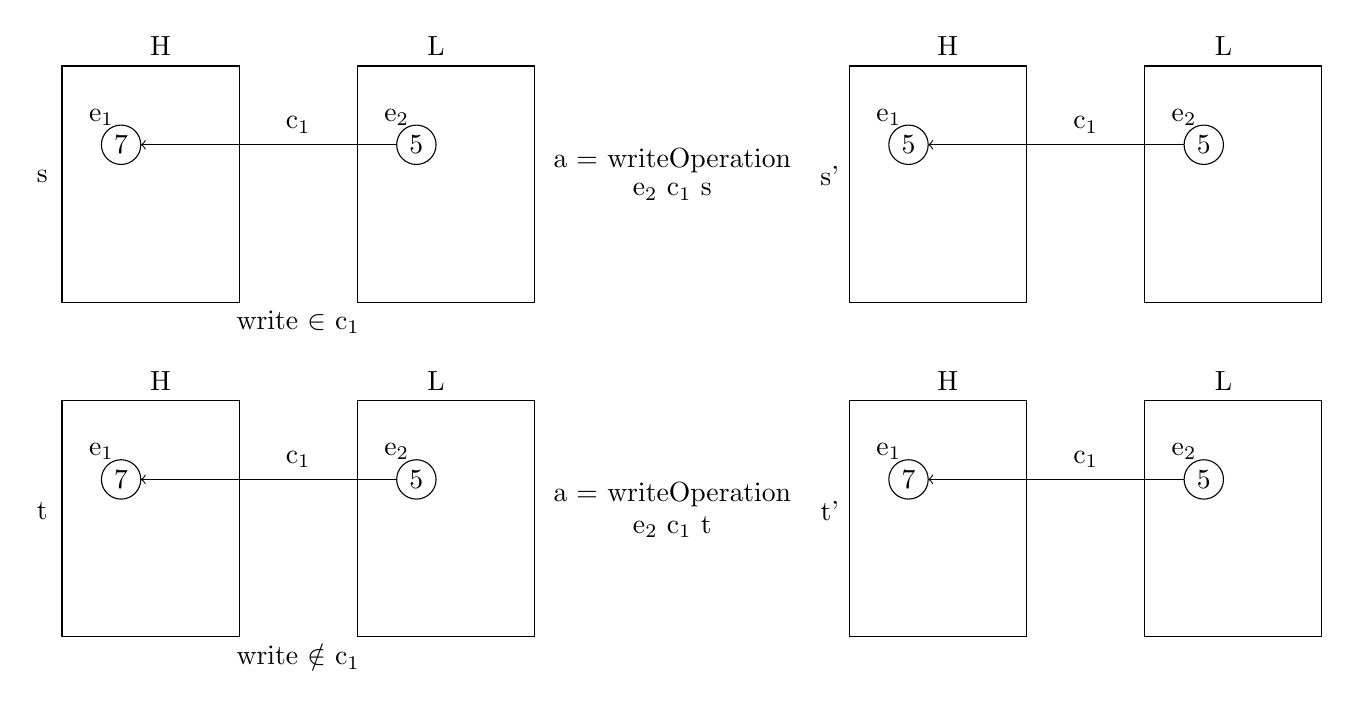
\begin{tikzpicture}
\node at (0,1.6) {t};
\node at (1.5,3.25) {H};
\draw [black] (0.25,0) rectangle (2.5,3);
\draw [black] (1,2) circle [radius=0.25] node {7};
\node at (0.75,2.35) {e$_1$};
\node at (5,3.25) {L};
\draw [black] (4,0) rectangle (6.25,3);
\draw [black] (4.75,2) circle [radius=0.25] node {5};
\node at (4.5,2.35) {e$_2$};
\draw [<-, black] (1.25,2) -- (4.5,2);
\node at (3.25,2.25) {c$_1$};
\node at (3.25,-0.25) {write $\notin$ c$_1$};

\node at (8,1.8) {a = writeOperation}; 
\node at (8,1.4) {e$_2$ c$_1$ t};

\node at (10,1.6) {t'};
\node at (11.5,3.25) {H};
\draw [black] (10.25,0) rectangle (12.5,3);
\draw [black] (14,0) rectangle (16.25,3);
\draw [black] (11,2) circle [radius=0.25] node {7};
\node at (10.75,2.35) {e$_1$};
\node at (15,3.25) {L};
\draw [black] (14.75,2) circle [radius=0.25] node {5};
\node at (14.5,2.35) {e$_2$};
\draw [<-, black] (11.25,2) -- (14.5,2);
\node at (13.25,2.25) {c$_1$};

\node at (0,5.85) {s};
\node at (1.5,7.5) {H};
\draw [black] (0.25,4.25) rectangle (2.5,7.25);
\draw [black] (4,4.25) rectangle (6.25,7.25);
\draw [black] (1,6.25) circle [radius=0.25] node {7};
\node at (0.75,6.6) {e$_1$};
\node at (5,7.5) {L};
\draw [<-, black] (1.25,6.25) -- (4.5,6.25);
\node at (3.25,6.5) {c$_1$};
\draw [black] (4.75,6.25) circle [radius=0.25] node {5};
\node at (4.5,6.6) {e$_2$};
\node at (3.25,4) {write $\in$ c$_1$};

\node at (8,6.05) {a = writeOperation};
\node at (8,5.65) {e$_2$ c$_1$ s};

\node at (10,5.85) {s'};
\node at (11.5,7.5) {H};
\draw [black] (10.25,4.25) rectangle (12.5,7.25);
\draw [black] (14,4.25) rectangle (16.25,7.25);
\draw [black] (11,6.25) circle [radius=0.25] node {5};
\node at (10.75,6.6) {e$_1$};
\node at (15,7.5) {L};
\draw [<-, black] (11.25,6.25) -- (14.5,6.25);
\node at (13.25,6.5) {c$_1$};
\draw [black] (14.75,6.25) circle [radius=0.25] node {5};
\node at (14.5,6.6) {e$_2$};
\end{tikzpicture}
\end{document}
